\documentclass[11pt,letterpaper]{article}
\usepackage[utf8]{inputenc}
\usepackage[top=1in,bottom=1in,left=1in,right=1in]{geometry}
\usepackage{amsmath}
\usepackage{amsfonts}
\usepackage{amssymb}
\usepackage{amsthm}
\usepackage{bm}
\usepackage{braket}
\usepackage{cancel}
\usepackage{enumitem}
\usepackage{float}
\usepackage[T1]{fontenc}
\usepackage{forloop}
\usepackage{graphicx}
\usepackage{hyperref}
\usepackage{lmodern}
\usepackage{mathabx}
\usepackage{parskip}
\usepackage{subcaption}
\usepackage{tensor}
\usepackage{titlesec}
\usepackage{titling}
\usepackage{listings}

\lstset{basicstyle=\footnotesize\ttfamily}

\setenumerate{leftmargin=*}


% \titlelabel{(\thetitle)\quad}
\titleformat*{\section}{\large\bfseries}
\titleformat*{\subsection}{\normalsize\bfseries}
\setlength{\droptitle}{-5em}


\DeclareMathOperator*{\argmin}{arg\,min}
\DeclareMathOperator*{\argmax}{arg\,max}

\DeclareMathOperator{\tr}{tr}

\let\Re\relax
\DeclareMathOperator{\Re}{Re}
\let\Im\relax
\DeclareMathOperator{\Im}{Im}

\DeclareMathOperator{\sgn}{sgn}

\newcommand{\R}{\mathbb{R}}


\theoremstyle{definition}
\newtheorem{defn}{Definition}[section]

\theoremstyle{plain}
\newtheorem{thm}{Theorem}[section]



\newcommand{\bhat}[1]{\hat{\bm{#1}}}
\newcommand{\prop}{\mathrel{\propto}}


\renewcommand{\thesubsection}{\normalsize \alph{subsection}}
\renewcommand{\d}{\mathrm{d}}
\renewcommand{\vec}[1]{\bm{#1}}
\newcommand{\del}{\vec{\nabla}}
\newcommand{\e}{\epsilon}
\newcommand{\tpd}[3]{\left( \frac{\partial #1}{\partial #2} \right)_{#3}}
\newcommand{\pd}[2]{\frac{\partial #1}{\partial #2}}
\newcommand{\spd}[2]{\frac{\partial^2 #1}{\partial {#2}^2}}
\def\dbar{{\mathchar'26\mkern-12mu d}}

\allowdisplaybreaks


\author{Sam Kowash}
\numberwithin{equation}{section}
\numberwithin{figure}{section}
\title{CSE 546 HW \#3}

\begin{document}
\maketitle

\section{Bayesian Inference}
\begin{enumerate}
	\item We consider $\{(x_i,y_i)\}_{i=1}^n$ sampled i.i.d.\ from a joint distribution $P_{XY}$ over $\R^d \times \R$ satisfying ${y_i \sim \mathcal{N}(x_i^T w, \sigma^2)}$ for some $w \in \R^d$. For compactness, let $\vec{X} = [x_1,\ldots,x_n]^T$ and $\vec{y} = [y_1,\ldots,y_n]^T$.

	\begin{enumerate}
		\item Assume that $(\vec{X}^T \vec{X})^{-1}$ exists. The likelihood for $w$ given a draw $X,y$ is
		%
		\begin{align*}
			\mathcal{L}(w \mid \vec{X},\vec{y}) &= \left(2\pi\sigma^2\right)^{-\frac{n}{2}} \exp\left[-\frac{(\vec{y}-\vec{X}w)^T (\vec{y}-\vec{X}w)}{2\sigma^2}\right],
		\end{align*}
		%
		so the log likelihood is
		%
		\begin{align*}
			\log \mathcal{L}(w \mid \vec{X},\vec{y}) &= -\frac{(\vec{y}-\vec{X}w)^T (\vec{y}-\vec{X}w)}{2\sigma^2} + \frac{n}{2} \ln (2\pi \sigma^2).
		\end{align*}
		%
		Setting the gradient with respect to $w$ to zero,
		%
		\begin{align*}
			0 &= -\frac{-2 \vec{X}^T \vec{y} + 2 \vec{X}^T \vec{X} w}{2\sigma^2}\\
			\vec{X}^T \vec{X} w &= \vec{X}^T \vec{y}\\
			\hat{w}_\mathrm{MLE} &= (\vec{X}^T \vec{X})^{-1} \vec{X}^T \vec{y}.
		\end{align*}



		\item If we assume that $w$ is actually drawn from a Gaussian prior
		%
		\begin{align*}
			p(w) &= \frac{1}{(2\pi\tau^2)^\frac{d}{2}} \exp\left[-\frac{\|w\|_2^2}{2\tau^2}\right],
		\end{align*}
		%
		then we can write down the posterior distribution (up to a positive constant)
		%
		\begin{align*}
			p(w \mid \vec{X},\vec{y}) &\prop p(\vec{X},\vec{y} \mid w) p(w)\\
			p(w \mid \vec{X},\vec{y}) &\prop \frac{1}{\sqrt{(2\pi\sigma^2)^n (2\pi \tau^2)}} \exp\left[-\frac{(\vec{y} - \vec{X}w)^T(\vec{y} - \vec{X}w)}{2\sigma^2} - \frac{w^T w}{2\tau^2}\right].
		\end{align*}
		%
		Absorbing the prefactor into the proportionality and taking a log, we get
		%
		\begin{align*}
			\log p(w \mid \vec{X},\vec{y}) &\prop -\frac{(\vec{y} - \vec{X}w)^T(\vec{y} - \vec{X}w)}{2\sigma^2} - \frac{w^T w}{2\tau^2},
		\end{align*}
		%
		which can be rearranged into the suggestive form
		%
		\begin{align*}
			\log p(w \mid \vec{X},\vec{y}) &\prop - \frac{\vec{y}^T \vec{y}}{2\sigma^2} + \frac{w^T \vec{X} \vec{y} + \vec{y}^T \vec{X}^T w}{2\sigma^2} - w^T \left(\frac{\vec{X}^T \vec{X}}{2\sigma^2} + \frac{I}{2\tau^2}\right) w.
		\end{align*}
		%
		Then, setting the gradient to zero,
		%
		\begin{align*}
			0 &= \frac{\vec{X}^T \vec{y}}{\sigma^2} - \left(\frac{\vec{X}^T \vec{X}}{\sigma^2} + \frac{I}{\tau^2}\right)w\\
			\vec{X}^T \vec{y} &= \left(\vec{X}^T \vec{X} + \frac{\sigma^2}{\tau^2} \right) w\\
			\hat{w}_\mathrm{MAP} &= \left(\vec{X}^T \vec{X} + \frac{\sigma^2}{\tau^2}\right)^{-1} \vec{X}^T \vec{y}.
		\end{align*}



		\item We can manipulate our previous proportionality expression
		%
		\begin{align*}
			p(w\mid \vec{X},\vec{y}) &\prop \exp\left[-\frac{(\vec{y} - \vec{X}w)^T(\vec{y} - \vec{X}w)}{2\sigma^2} - \frac{w^T w}{2\tau^2}\right]
		\end{align*}
		%
		to determine the exact form of the posterior distribution. The objective will be to complete the square into a single Gaussian in $w$. First, multiplying out,
		%
		\begin{align*}
			p(w\mid \vec{X},\vec{y}) &\prop \exp\left\{-\frac{1}{2}\left[w^T \left(\frac{\vec{X}^T \vec{X}}{\sigma^2} + \frac{I}{\tau^2}\right)w - \frac{2\vec{y}^T \vec{X} w}{\sigma^2} - \frac{\vec{y}^T \vec{y}}{\sigma^2}\right]\right\}.
		\end{align*}
		%
		We want to find a $\mu$ such that
		%
		\begin{align*}
			(w-\mu)^T \left(\frac{\vec{X}^T \vec{X}}{\sigma^2} + \frac{I}{\tau^2}\right) (w-\mu)
		\end{align*}
		%
		produces the correct cross-term in $w$. Expanding this expression gives,
		%
		\begin{align*}
			(w-\mu)^T \left(\frac{\vec{X}^T \vec{X}}{\sigma^2} + \frac{I}{\tau^2}\right) (w-\mu) &= w^T \left(\frac{\vec{X}^T \vec{X}}{\sigma^2} + \frac{I}{\tau^2}\right)w - 2\mu^T \left(\frac{\vec{X}^T \vec{X}}{\sigma^2} + \frac{I}{\tau^2}\right) w\\&\quad + \mu^T \left(\frac{\vec{X}^T \vec{X}}{\sigma^2} + \frac{I}{\tau^2}\right) \mu,
		\end{align*}
		%
		which means $\mu$ must satisfy
		%
		\begin{align*}
			\mu^T \left(\frac{\vec{X}^T \vec{X}}{\sigma^2} + \frac{I}{\tau^2}\right) w &= \frac{\vec{y}^T \vec{X}}{\sigma^2} w.
		\end{align*}
		%
		Since this must hold for all $w$, we find
		%
		\begin{align*}
			\mu^T &=  \frac{\vec{y}^T \vec{X}}{\sigma^2}\left(\frac{\vec{X}^T \vec{X}}{\sigma^2} + \frac{I}{\tau^2}\right)^{-1}\\
			\mu &= \left(\vec{X}^T \vec{X} + \frac{\sigma^2}{\tau^2}\right)^{-1} \vec{X}^T \vec{y},
		\end{align*}
		%
		which is exactly our MAP estimator, unsurprisingly. Defining
		%
		\begin{align*}
			\Sigma &= \left(\frac{\vec{X}^T \vec{X}}{\sigma^2} + \frac{I}{\tau^2}\right)^{-1},
		\end{align*}
		%
		we can see that
		%
		\begin{align*}
			p(w \mid \vec{X},\vec{y}) &\prop \exp\left\{-\frac{1}{2}\left[(w-\mu)^T \Sigma^{-1} (w-\mu) - \mu^T \Sigma^{-1} \mu - \frac{\vec{y}^T \vec{y}}{\sigma^2}\right]\right\},
		\end{align*}
		%
		and since the second and third terms in the exponential have no dependence on $w$, indeed
		%
		\begin{align*}
			p(w \mid \vec{X},\vec{y}) &\prop \exp\left\{-\frac{1}{2}(w-\mu)^T \Sigma^{-1} (w-\mu)\right\}.
		\end{align*}
		%
		This is the full $w$-dependence of the distribution, and the constant of proportionality only enforces normalization, so we conclude that $p(w\mid \vec{X},\vec{y}) \sim \mathcal{N}(\mu,\Sigma)$ as defined above.

		\item We now fix $z \in \R^d$ and define $f_z = z^T w$ as the predicted function value at $z$. Given the previous result, and knowing that affine transformations of normal random variables are themselves normal with $\mu$ and $\Sigma$ transformed accordingly, we can see that
		%
		\begin{align*}
			f_z \mid \vec{X},\vec{y} &\sim \mathcal{N}\left(z^T \mu, z^T \Sigma z\right),
		\end{align*}
		%
		or, explicitly,
		%
		\begin{align*}
			f_z \mid \vec{X},\vec{y} &\sim \mathcal{N}\left(z^T \left(\vec{X}^T \vec{X} + \tfrac{\sigma^2}{\tau^2}\right)^{-1} \vec{X}^T \vec{y}, z^T \left(\tfrac{\vec{X}^T \vec{X}}{\sigma^2} + \tfrac{I}{\tau^2}\right)^{-1} z\right)\\
			f_z \mid \vec{X},\vec{y} &\sim \mathcal{N}\left(z^T \left(\vec{X}^T \vec{X} + \tfrac{\sigma^2}{\tau^2}\right)^{-1} \vec{X}^T \vec{y}, \sigma^2 z^T \left(\vec{X}^T \vec{X} + \tfrac{\sigma^2}{\tau^2}\right)^{-1} z\right).
		\end{align*}




		\item It is an identity that for matrices $A,U,C,V$ with $A$ nonsingular, we have
		%
		\begin{align*}
			(A+UCV)^{-1} &= A^{-1} - A^{-1}U\left(C^{-1} + V A^{-1} U \right)^{-1} V A^{-1}.
		\end{align*}
		%
		Taking
		%
		\begin{align*}
			A &= \frac{\sigma^2}{\tau^2} I\\
			U &= \vec{X}^T\\
			C &= I\\
			V &= \vec{X},
		\end{align*}
		%
		we get
		%
		\begin{align*}
			\left(\frac{\sigma^2}{\tau^2} I + \vec{X}^T \vec{X}\right)^{-1} &= \frac{\tau^2}{\sigma^2} I - \frac{\tau^2}{\sigma^2} \vec{X}^T \left(I + \vec{X} \frac{\tau^2}{\sigma^2} \vec{X}^T\right)^{-1} \vec{X} \frac{\tau^2}{\sigma^2}\\
			\left(\frac{\sigma^2}{\tau^2} I + \vec{X}^T \vec{X}\right)^{-1} &= \frac{\tau^2}{\sigma^2} I - \frac{\tau^2}{\sigma^2} \vec{X}^T \left(\frac{\sigma^2}{\tau^2} I + \vec{X}\vec{X}^T\right)^{-1} \vec{X}.
		\end{align*}
		%
		Now defining
		%
		\begin{align*}
			\vec{K} &= \vec{X}\vec{X}^T\\
			\vec{k}_{\cdot z} &= \vec{X} z\\
			k_{zz} &= z^T z,
		\end{align*}
		%
		we can rewrite $z^T \mu$ as
		%
		\begin{align*}
			z^T \mu = z^T \left(\vec{X}^T \vec{X} + \frac{\sigma^2}{\tau^2}\right)^{-1} \vec{X}^T \vec{y} &= \frac{\tau^2}{\sigma^2} z^T \left[I - \vec{X}^T \left(\frac{\sigma^2}{\tau^2} I + \vec{X} \vec{X}^T\right)^{-1} \vec{X}\right]\vec{X}^T \vec{y}\\
			%
			z^T \mu &= \frac{\tau^2}{\sigma^2} \left[\vec{k}_{\cdot z}^T \vec{y} - \vec{k}_{\cdot z}^T \left(\frac{\sigma^2}{\tau^2}I + \vec{K}\right)^{-1} \vec{K} \vec{y}\right].
		\end{align*}
		%
		If we insert an identity in the middle of the first term as $(\tfrac{\sigma^2}{\tau^2} I + \vec{K})^{-1} (\tfrac{\sigma^2}{\tau^2} I + \vec{K})$, then
		%
		\begin{align*}
			z^T \mu &= \frac{\tau^2}{\sigma^2} \vec{k}_{\cdot z}^T \left(\frac{\sigma^2}{\tau^2} I + \vec{K}\right)^{-1} \left[\frac{\sigma^2}{\tau^2} I + \vec{K} - \vec{K}\right]\vec{y}\\
			z^T \mu &= \vec{k}_{\cdot z}^T \left(\frac{\sigma^2}{\tau^2} I + \vec{K}\right)^{-1} \!\!\! \vec{y}.
		\end{align*}
		%
		Similarly, we can rewrite the variance (in fewer steps) as
		%
		\begin{align*}
			\sigma^2 z^T \Sigma z = \sigma^2 z^T \left(\vec{X}^T \vec{X} + \tfrac{\sigma^2}{\tau^2}\right)^{-1} z &= \tau^2 \left[k_{zz} - \vec{k}_{\cdot z}^T \left(\tfrac{\sigma^2}{\tau^2} I + \vec{K}\right)^{-1}\vec{k}_{\cdot z}\right].
		\end{align*}
		%
		We then see that our MAP estimate (the mean of this distribution) for $f_z$ is exactly the prediction made by kernel ridge regression with a linear kernel given by $K$ and regularization $\sigma^2/\tau^2$.
	\end{enumerate}






	\item Let $\{(x_i, y_i)\}_{i=1}^n$ be drawn i.i.d.\ from a distribution $P_{XY}$ over $\R^d \times \R$ such that for some $w \in \R^d$ we have $y_i \sim \mathcal{N}(x_i^T w, \sigma^2)$. 
	%
	\begin{enumerate}
		\item Suppose that $w$ is drawn from a Laplace prior
		%
		\begin{align*}
			p(w) &= \frac{1}{(2a)^d} \exp\left(-\frac{\|w\|_1}{a}\right).
		\end{align*}
		%
		The posterior distribution then satisfies
		%
		\begin{align*}
			p(w \mid \vec{X},\vec{y}) &\prop \exp\left[-\frac{(\vec{y} - \vec{X}w)^T(\vec{y} - \vec{X} w)}{2\sigma^2} - \frac{\|w\|_1}{a}\right].
		\end{align*}
		%
		Maximizing this probability is minimizing
		%
		\begin{align*}
			\frac{(\vec{y} - \vec{X}w)^T(\vec{y} - \vec{X} w)}{2\sigma^2} + \frac{\|w\|_1}{a},
		\end{align*}
		%
		which is LASSO regression with $\lambda  = 1/a$. We know that this does not have a general closed form for $d>1$ so can say simply
		%
		\begin{align*}
			\hat{w}_\mathrm{MAP} &= \hat{w}_\mathrm{LASSO},
		\end{align*}
		%
		and use our existing coordinate descent algorithm based on the subgradient of the LASSO objective to find particular solutions.


		\item 
	\end{enumerate}
\end{enumerate}
































\section{Kernel Regression}
\begin{enumerate}
\setcounter{enumi}{2}
	\item \begin{enumerate}
		\item Leave-one-out cross-validation with random search gave $\lambda = 2.66\times10^{-7}$ and $d=18$ for the polynomial kernel. Similarly, for the RBF kernel we get $\lambda = 4.94\times10^{-4}$ and $\gamma = 25.82$.

		\item 

		\begin{figure}[H]
			\centering
			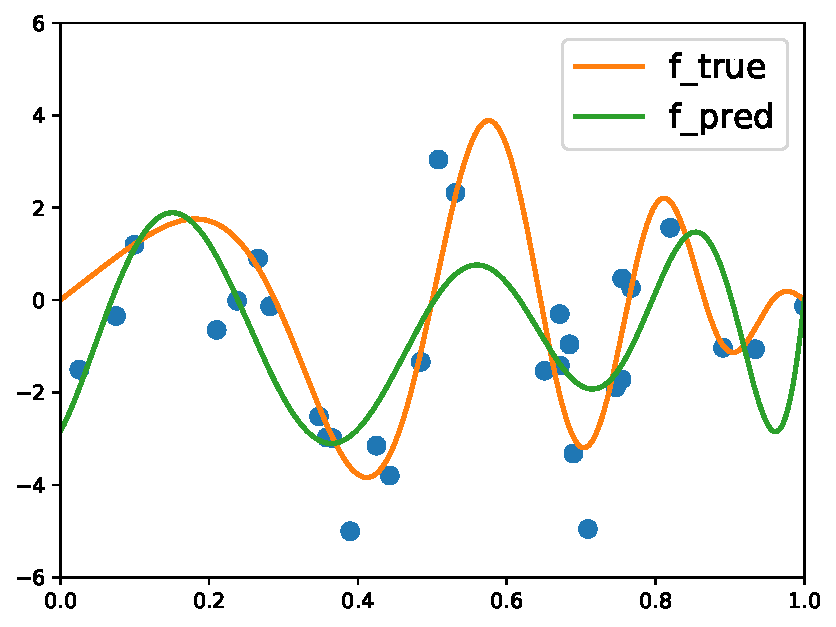
\includegraphics[width=.6\textwidth]{figures/poly_ker_d20_lm4.pdf}
			\caption{Predicted and actual functions with polynomial kernel, $d=20$, $\lambda = 10^{-4}$}
		\end{figure}

		\begin{figure}[H]
			\centering
			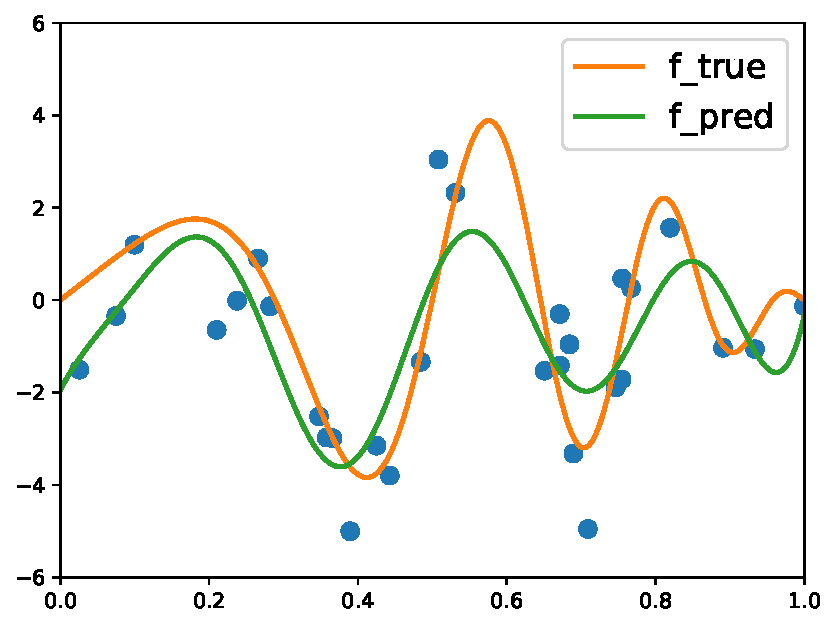
\includegraphics[width=.6\textwidth]{figures/rbf_ker_gp5_lm4.pdf}
			\caption{Predicted and actual functions with rbf kernel, $\gamma = 10$, $\lambda = 10^{-4}$}
		\end{figure}
		\item 
		\item 
		\item 
	\end{enumerate}
\end{enumerate}




















\section{\texorpdfstring{$k$-means clustering}{k-means clustering}}
\begin{enumerate}
\setcounter{enumi}{3}
	\item \begin{enumerate}
		\item Figures below show cluster centers in the full MNIST set (train joined with test) from $k$-means for a variety of different cluster counts. In general, they all resemble identifiable numerals, but more clusters tends to lead to more distinct features. At $k=5$ we see centers somewhere in between similar numerals like 3 and 8 or 9 and 4, but at $k=20$ the algorithm has the freedom to center clusters around more specific forms like taller or rounder or more slanted 9s.


		\begin{figure}[H]
			\centering
			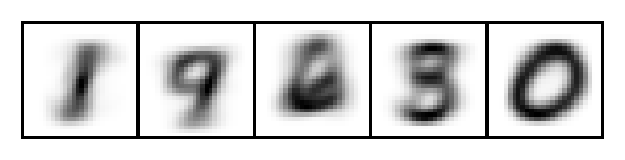
\includegraphics[width=.5\textwidth]{figures/5-centers.pdf}
			\caption{Final centers for $k=5$ with uniform initialization}
		\end{figure}

		\begin{figure}[H]
			\centering
			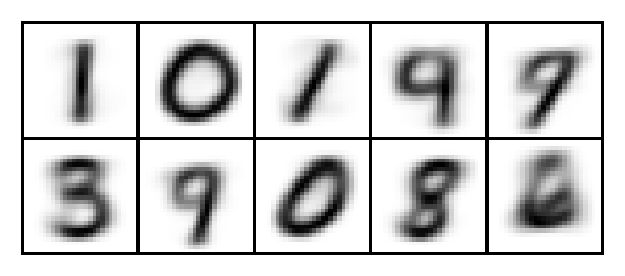
\includegraphics[width=.5\textwidth]{figures/10-centers.pdf}
			\caption{Final centers for $k=10$ with uniform initialization}
		\end{figure}

		\begin{figure}[H]
			\centering
			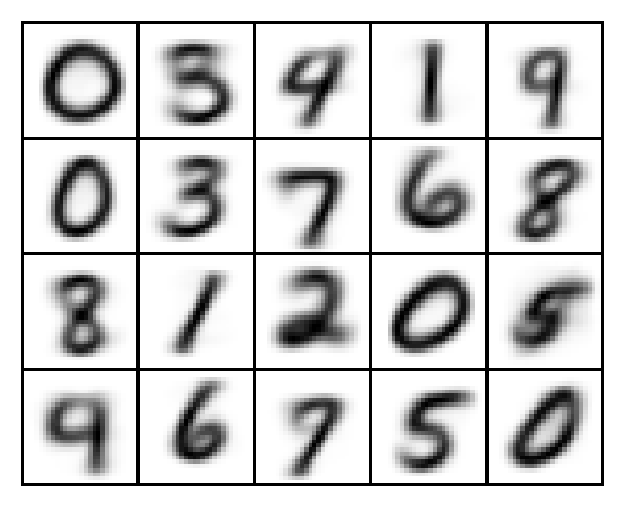
\includegraphics[width=.5\textwidth]{figures/20-centers.pdf}
			\caption{Final centers for $k=20$ with uniform initialization}
		\end{figure}




		\item Figures below show centers obtained with the $\texttt{k-means++}$ intialization scheme. They look broadly similar to the uniform case, although perhaps modestly crisper. 

		Fig.~\ref{fig:km_objs} compare the convergence rate to uniform initialization through the mean squared distance from a point to its cluster center. We see that other than for $k=5$, the new initialization converges faster and to smaller mean distances.

		\begin{figure}[H]
			\centering
			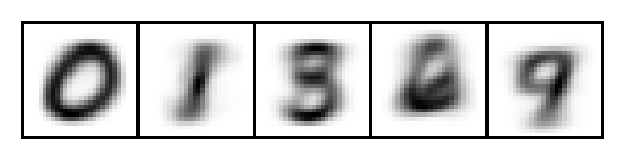
\includegraphics[width=.5\textwidth]{figures/5pp-centers.pdf}
			\caption{Final centers for $k=5$ with \texttt{k-means++} initialization}
		\end{figure}

		\begin{figure}[H]
			\centering
			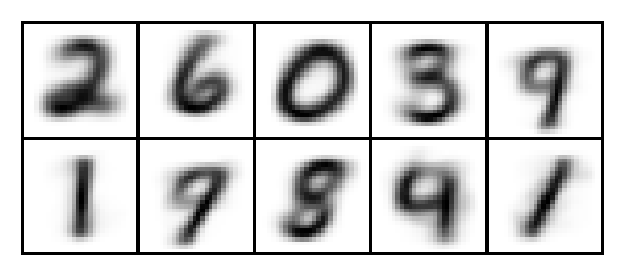
\includegraphics[width=.5\textwidth]{figures/10pp-centers.pdf}
			\caption{Final centers for $k=10$ with \texttt{k-means++} initialization}
		\end{figure}

		\begin{figure}[H]
			\centering
			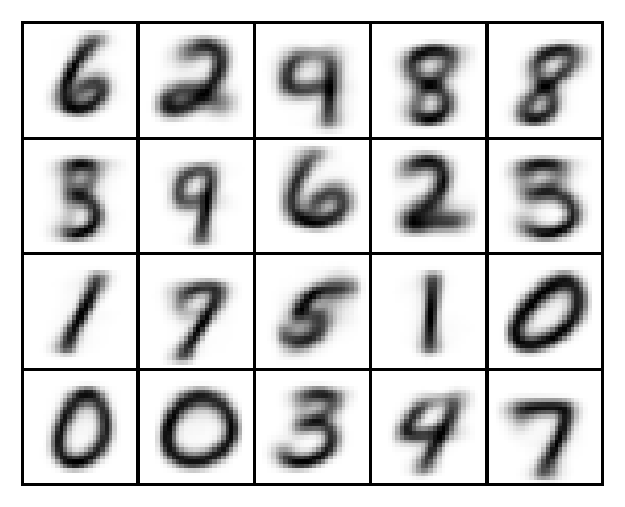
\includegraphics[width=.5\textwidth]{figures/20pp-centers.pdf}
			\caption{Final centers for $k=20$ with \texttt{k-means++} initialization}
		\end{figure}


		\begin{figure}[H]
		\centering
			\begin{subfigure}[t]{.32\textwidth}
				\centering
				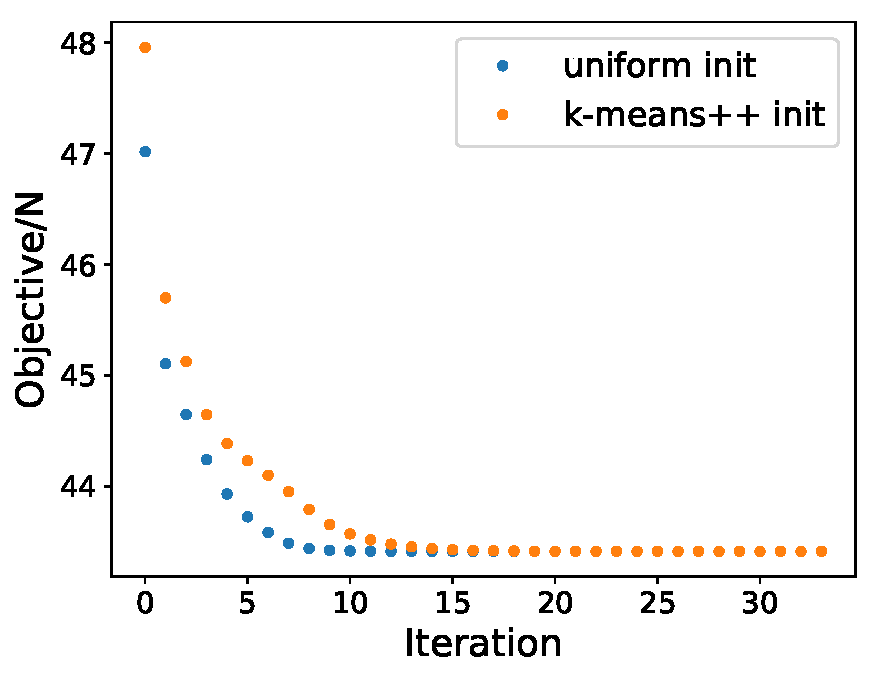
\includegraphics[width=\textwidth]{figures/5-objective.pdf}
			\end{subfigure}
			%
			\begin{subfigure}[t]{.32\textwidth}
				\centering
				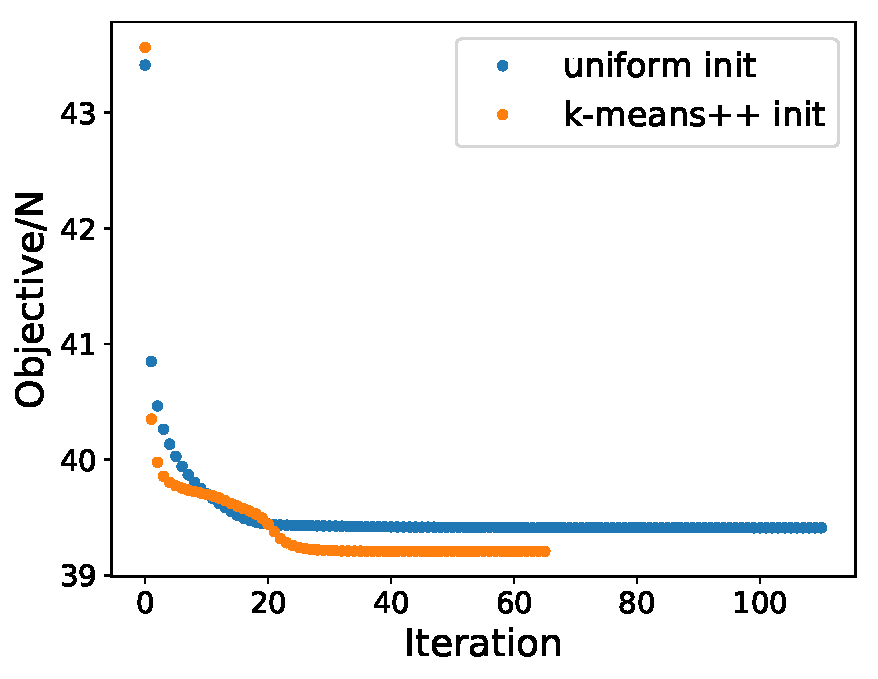
\includegraphics[width=\textwidth]{figures/10-objective.pdf}
			\end{subfigure}
			%
			\begin{subfigure}[t]{.32\textwidth}
				\centering
				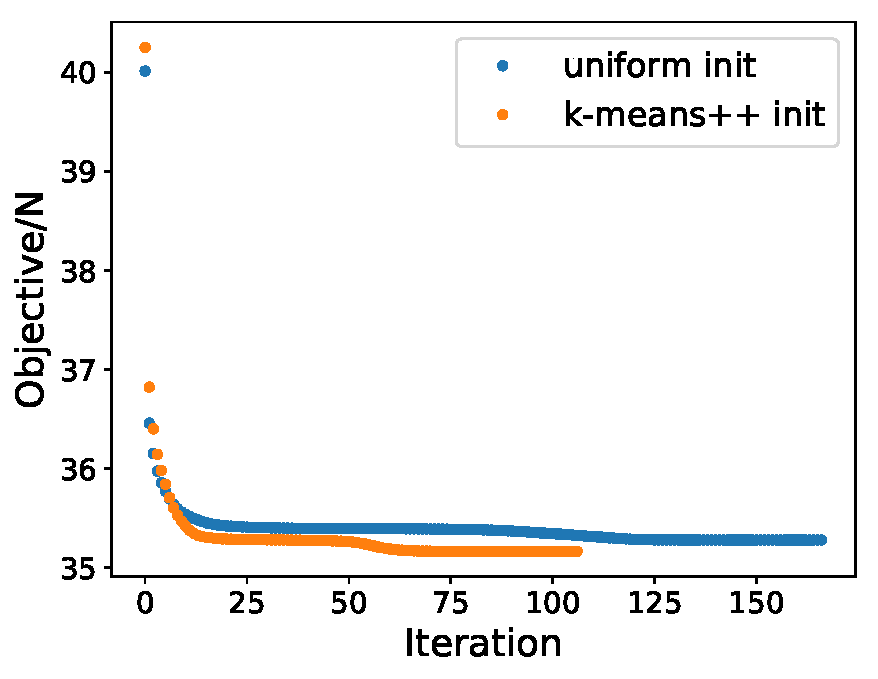
\includegraphics[width=\textwidth]{figures/20-objective.pdf}
			\end{subfigure}

			\caption{Objective function vs. iteration number for $k = 5,10,20$ from left to right}
		\end{figure}
		\label{fig:km_objs}
	\end{enumerate}
\end{enumerate}
















\section{Joke Recommender System}
\begin{enumerate}
\setcounter{enumi}{4}
	\item \begin{enumerate}
		\item
		\item 
		\item 
	\end{enumerate}
\end{enumerate}





\clearpage
\lstinputlisting[language=Python]{code/kernreg.py}
\clearpage
\lstinputlisting[language=Python]{code/plotter.py}
\clearpage
\lstinputlisting[language=Python]{code/kmeans.py}
\clearpage
\lstinputlisting[language=Python]{code/jester.py}


\end{document}